% - neutrino detectors
\section{Neutrino detection}

You cannot see a neutrino directly, but if it interacts with a particle in our detector, we might observe and identify the byproducts of the interaction.
A few techniques to determine neutrino fluxes and study neutrino's interactions with other particles have been developped.
This section lists some of these methods.

\subsection{Counting atoms}
When neutrinos interact with the neutrons in the atom, a lepton and a proton may be produced
\begin{equation*}
  \nu_e + n \to e^- + p^+,
\end{equation*}
changing the nuclear structure and chemical properties of the atom it interacted with.
If a tank is filled with pure homoatomic liquid and one is able to detect and count the resulting new atoms\marginnote{\emph{Chemists} know how to do this!} of the neutrino interactions, one can draw conclusions on the neutrinos and the neutrino flux.
If the production rate of neutrinos can be controlled, as it is the case with nuclear reactors, the results are even more evident.
And even though counting the number of atoms seems a difficult process, a number of experiments proove that it is feasable.\marginnote{Like the experiment run by John Bahcall and Raymond Davis Jr.}

\subsection{Observing chain interactions}
One could observe the subsequent reactions of the byproducts of the neutrino interaction\marginnote{This astute technique was used by Clyde Cowan and Frederick Reines to detect electron antineutrinos.} to conclude a neutrino interaction.
A clear signal raising from the background is needed for this cause.
For instance, the interaction of an electron antineutrino and a proton results in a neutron and a positron
\begin{equation*}
  \bar{\nu}_e + p^+ \to n + e^+.
\end{equation*}
The positron won't travel very far in matter until it annihilates with an electron, emitting two photons
\begin{equation*}
  e^+ + e^- \to \gamma + \gamma
\end{equation*}
with an energy of approximately half an MeV\marginnote{In a center of mass system, the photons' energy will be equivalent to the electron and positron's mass.} in opposite directions.
If the neutron is absorbed by the nucleus of some atom, the latter may react.
When cadmium absorbs a neutron, it'll go into a meta-stable state, which decays into its ground state by emmiting a gamma ray
\begin{equation*}
  n + \ce{^{108}Cd} \to \ce{^{109}Cd^*} \to \ce{^{109}Cd} + \gamma.
\end{equation*}
The time window from the neutrino interaction to the electron positron annihilation and the gamma emission of the nucleus is a determinant characteristic of the process.

\subsection{Cherenkov detectors} No particle faster than the speed of light in vacuum\marginnote{Physicists call these hypothetical particles \emph{tachions}.} was found so far.
But light's speed depends on the refractive index of the medium it is travelling through.
Therefore charged particles can travel through a suitable medium faster than light does, producing \emph{Cherenkov radiation}, a measurable cone of light.
This light can be read out to reconstruct the geometry of the cone and identify the particle which generated it.
Such cones are displayed in the illustrations of figure \ref{fig:super_kamiokande_events}.
Kamiokande, \gls{lsnd}, MiniBooNE and many other detectors used this technique.

\begin{figure*}
  \centering
  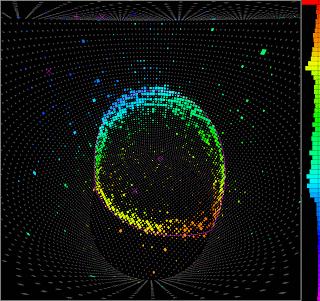
\includegraphics[width=.48\textwidth]{super_kamiokande/muon}
  \hspace*{1em}
  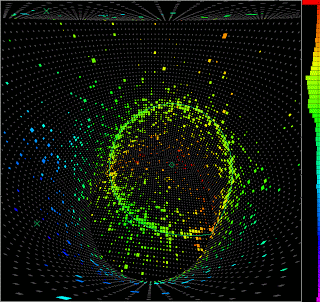
\includegraphics[width=.48\textwidth]{super_kamiokande/electron}
  \caption{%
    Images of events in Super Kamiokande.
    The illustration on the left shows a muon event, the one on the right an electron event.
    The muon's cone has a clean shape while the electron's cone is less evident.
    Electrons scatter more than muons, due to their lower mass, leading to a spread cone.
    The time scale of on the right displays the time window and energy deposit during the observation.
    -- \copyright Tomasz Barszczak - Super-Kamiokande Collaboration
  }
  \label{fig:super_kamiokande_events}
\end{figure*}

\subsection{Bubble \& cloud chambers} Another way to trace charged particles is by putting a fluid close to phase transition in their path.
When the charged particle interacts with the liquid, it produces heat, letting the fluid change its phase, such that bubbles will form.
Bubble chambers and cloud chambers use this effect to produce and image such traces.
The length, thickness and shape of the trace is determinant for the particle generating it.
To be able to reconstruct one event, several images from different angles are needed.
Figure \ref{fig:observation} is a good example of an interaction seen in such a detector.
\marginnote{Watch Professor Sumner Davis' \href{https://www.youtube.com/watch?v=HuIiKy_2F6g}{Advanced Laboratory on Bubble Chambers}}

\subsection{Photoemulsion films} Using a specially chosen chemical compound, which alters its state permanently after interacting with incident radiation, offers a further possibility to trace charged particles.
Photoemulsion films exploit this idea and lead to images like the one illustrated in figure \ref{fig:photoemulsion}.
The grains become visible after a development process, revealing the tracks left behind by the particles.
The OPERA experiment was able to proof the appearance of tauon neutrinos in a muon neutrino beam using this technique\cite{Ereditato2016116}.

\begin{figure}
  \centering
  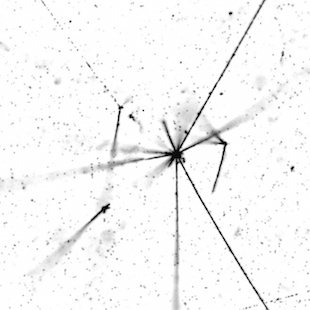
\includegraphics[width=.8\textwidth]{photoemulsion}
  \caption[][24.5em]{%
    Interaction of an anti-proton with a nucleon of an atom in a photo-emulsion film.
    The AEgIS experiment -- source of this event -- uses such emulsion films to measure the gravitational force on antihydrogen
    -- \copyright LHEP Universität Bern
  }
  \label{fig:photoemulsion}
\end{figure}

\subsection{Time projection chambers} In a medium the ionized atoms generated by the incident radiation recombine shortly after being ionized.
By applying an electric field, recombination can be supressed and the ionization electrons can be trapped, letting them drift through the fluid towards a charge collector.
The path can be reconstructed if the drift speed is constant and the time the particle was drifting is determined.
These kind of detectors are called \glspl{tpc}.
MicroBooNE, SBND and Icarus feature \gls{lartpc} in their apparati.
A few events as registered by the \glspl{lartpc} of MicroBooNE are displayed in figure \ref{fig:events_microboone}.

\begin{figure}
  \centering
  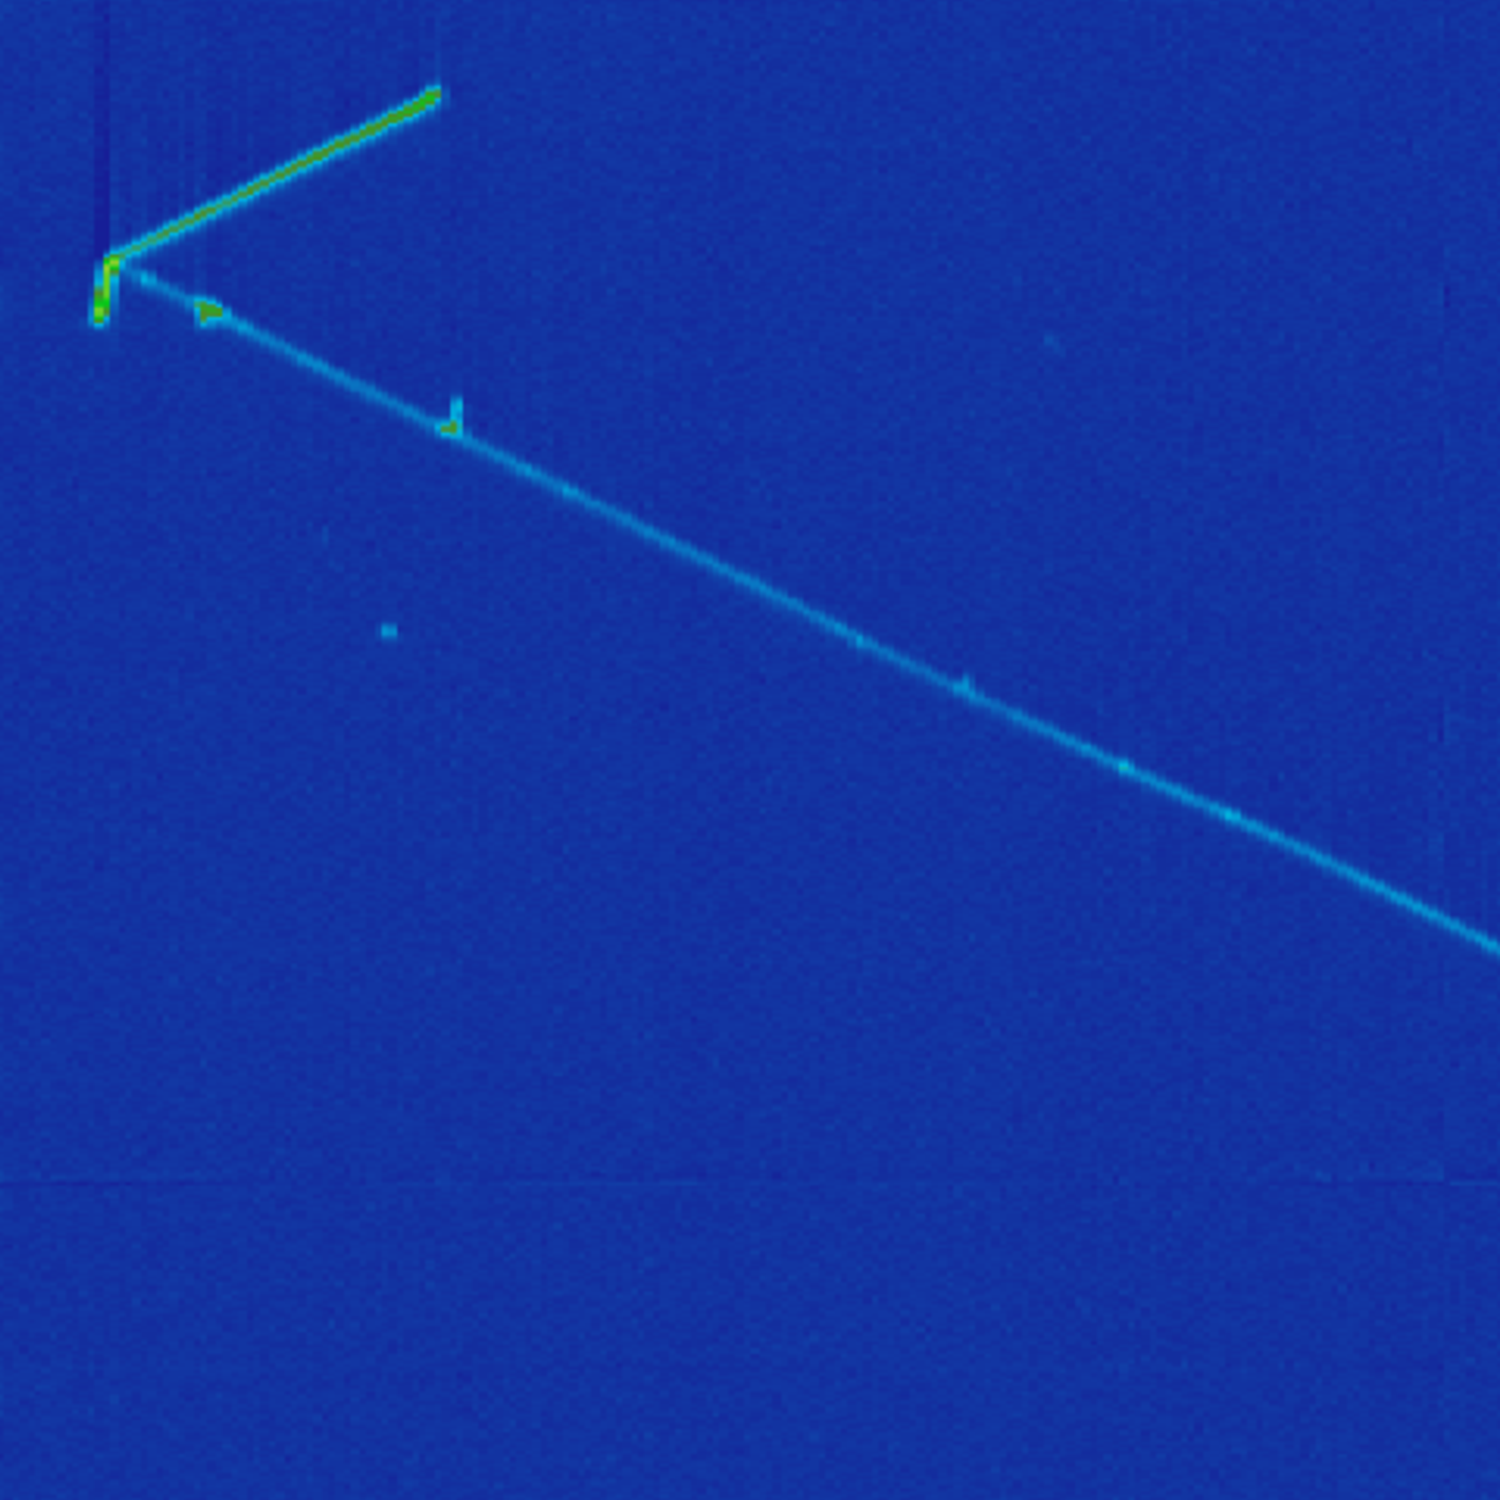
\includegraphics[width=.46\textwidth]{microboone_events/cut/ccqe}
  \hspace*{.5em}
  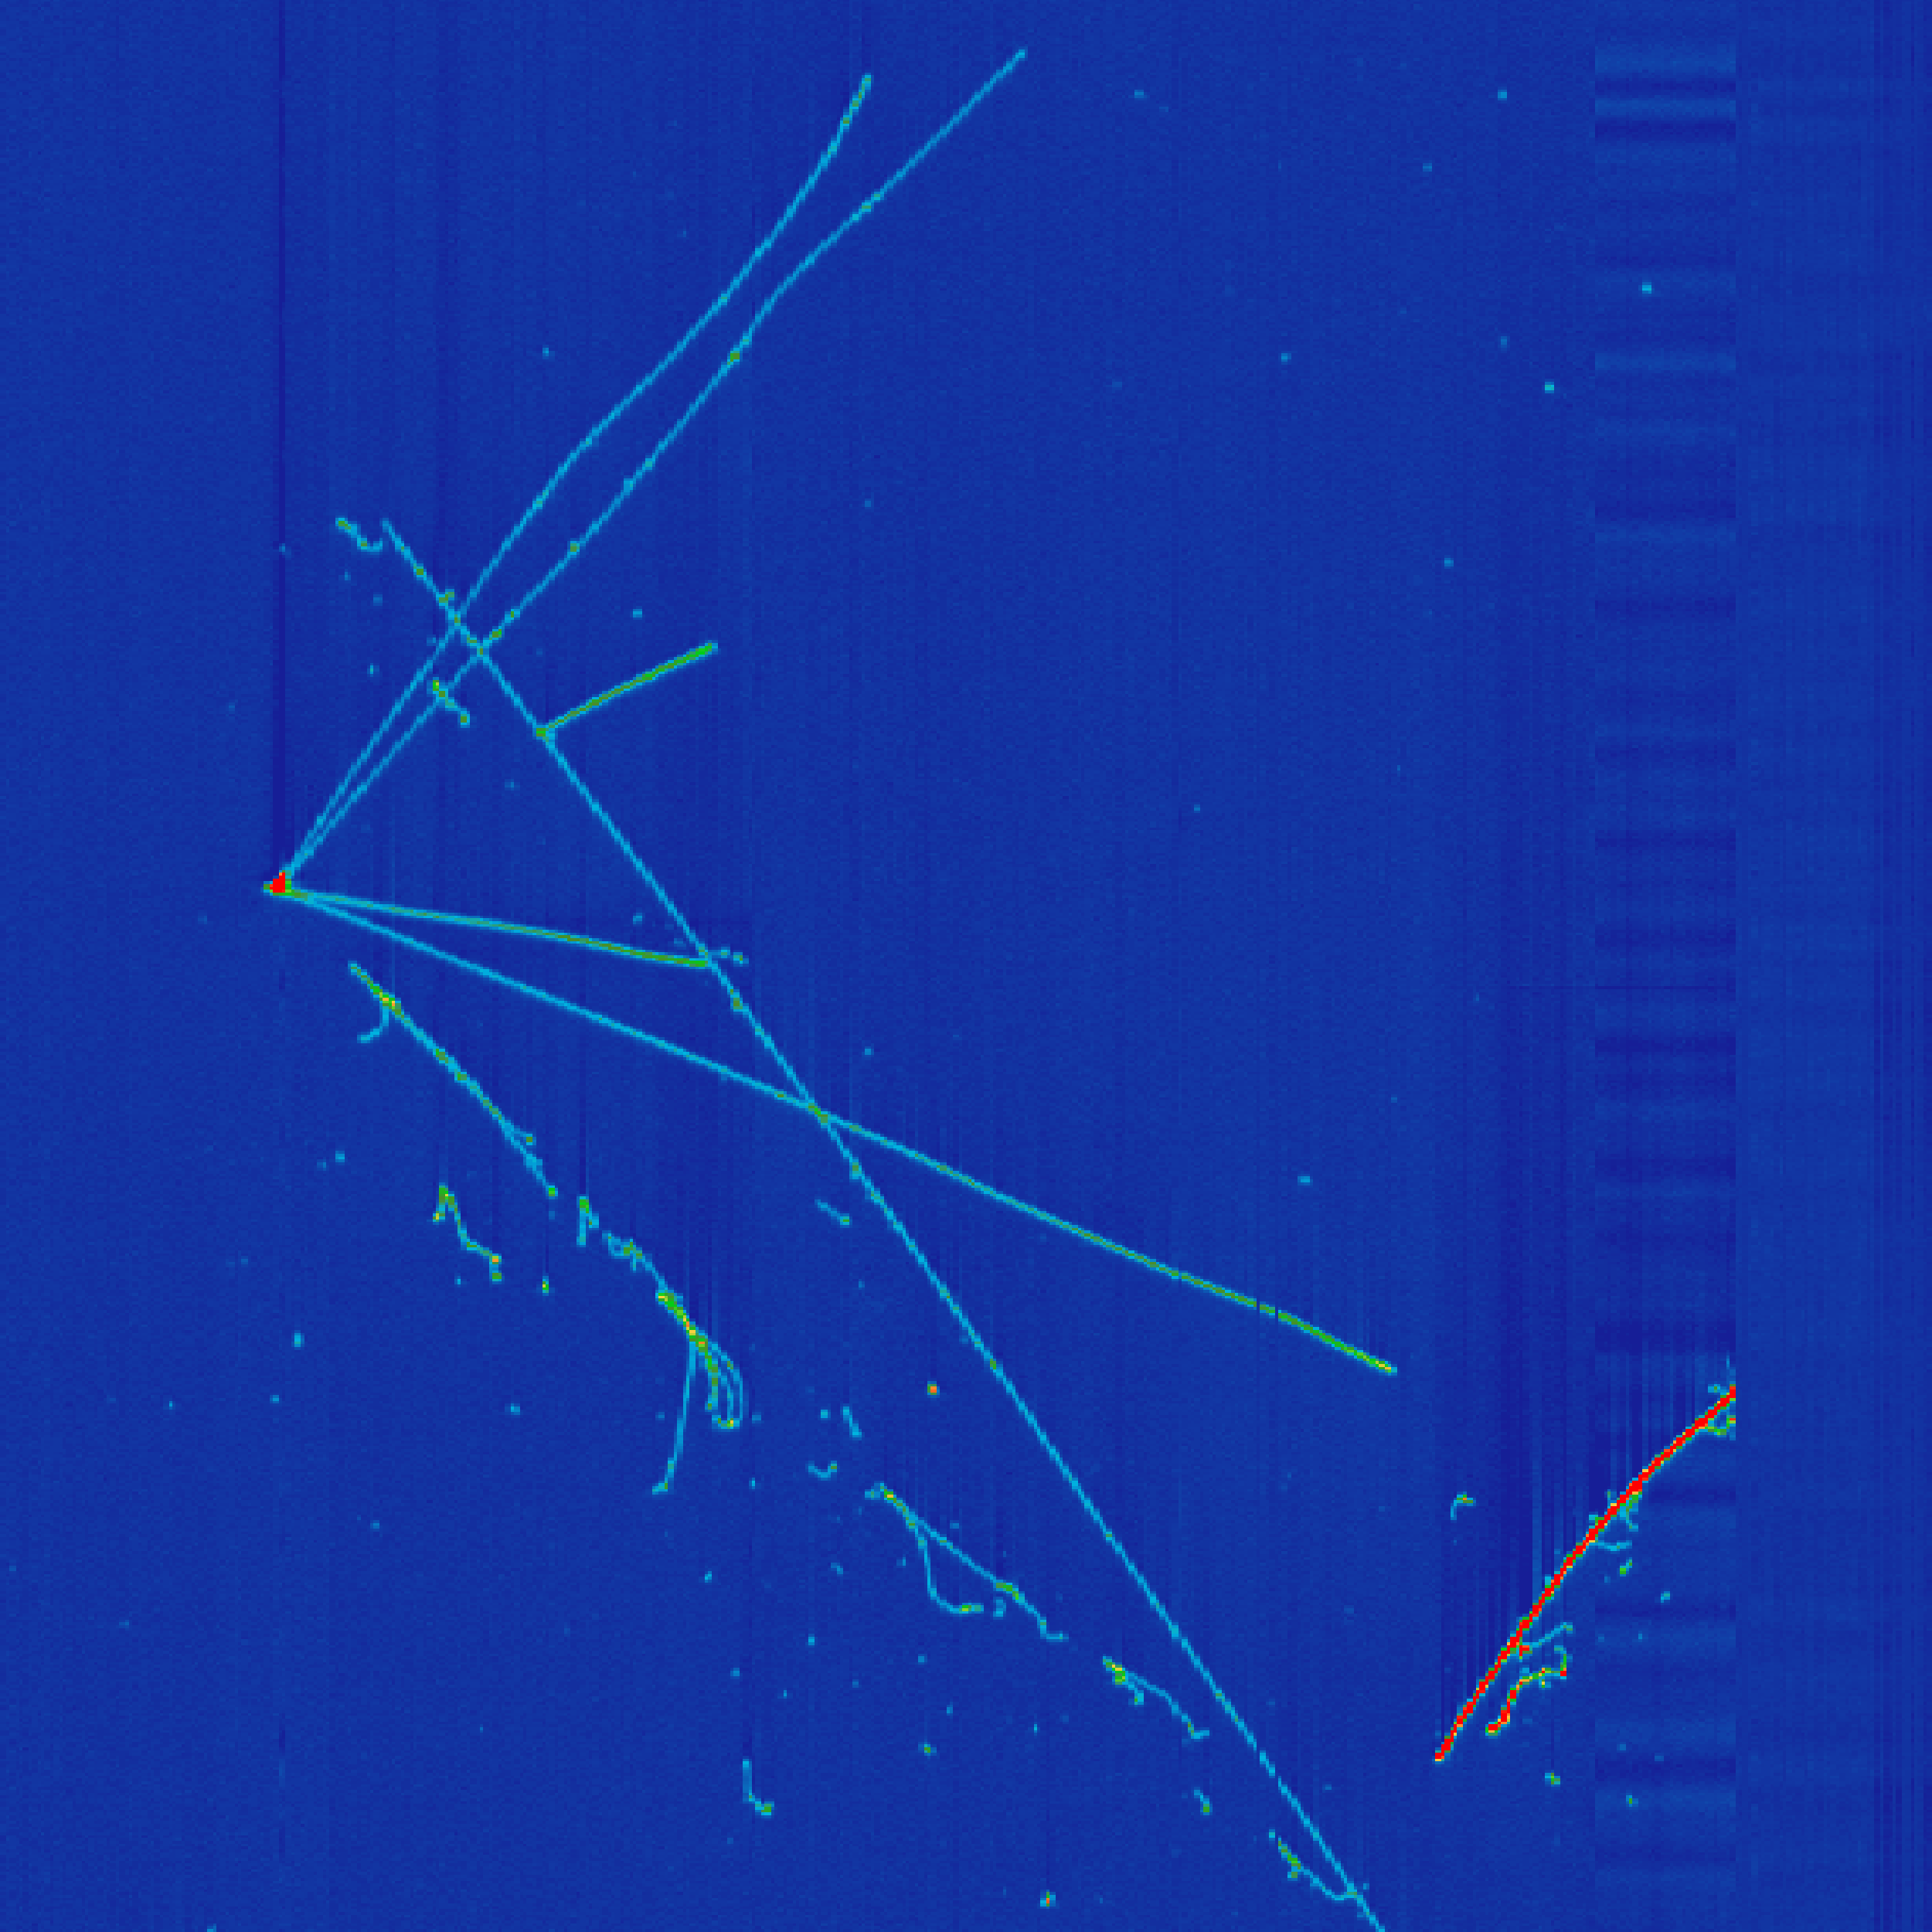
\includegraphics[width=.46\textwidth]{microboone_events/cut/dis}
  \caption{%
    The event on the left is a candidate of a quasi-elastic scattering event.
    The event on the right is probably a deep inelastic scattering event with a candidate of a cosmic ray.
    -- \copyright \href{http://www-microboone.fnal.gov/first-neutrinos/index.html}{fnal.gov}
  }
  \label{fig:events_microboone}
\end{figure}
